%%% template.tex
%%%
%%% This LaTeX source document can be used as the basis for your technical
%%% paper or abstract. Intentionally stripped of annotation, the parameters
%%% and commands should be adjusted for your particular paper - title, 
%%% author, article DOI, etc.
%%% The accompanying ``template.annotated.tex'' provides copious annotation
%%% for the commands and parameters found in the source document. (The code
%%% is identical in ``template.tex'' and ``template.annotated.tex.'')

\documentclass[conference]{acmsiggraph}

\usepackage{authblk}
\usepackage[]{algorithm2e}

\TOGonlineid{45678}
\TOGvolume{0}
\TOGnumber{0}
\TOGarticleDOI{1111111.2222222}
\TOGprojectURL{}
\TOGvideoURL{}
\TOGdataURL{}
\TOGcodeURL{}



\title{Tracking Objects on a Deformable Surface using Displacement and Orientation Information}

\author[1]{Zachary DeStefano\thanks{zdestefa@uci.edu}}
\author[1]{Kyle Cutler\thanks{kbcutler58@gmail.com}}
\author[1]{Gopi Meenakshisundaram\thanks{gopi.meenakshisundaram@gmail.com}}
\author[1]{Thomas O'Sullivan\thanks{tosulliv@uci.edu}}
\author[1]{Albert Cerussi\thanks{acerussi@apple.com}}
\author[1]{Bruce Tromberg\thanks{bjtrombe@uci.edu}}
\pdfauthor{Zachary DeStefano,Kyle Cutler,Gopi Meenakshisundaram,Thomas O'Sullivan, Albert Cerussi,Bruce Tromberg}
\affil[1]{University of California, Irvine}

\keywords{Tracking, Deformable Surface}

\begin{document}

%% \teaser{
%%   \includegraphics[height=1.5in]{images/sampleteaser}
%%   \caption{Spring Training 2009, Peoria, AZ.}
%% }

\maketitle



\section{Tracking the Probe on a Deformable Surface}

\subsection{Mesh Following Algorithm}

After calibration, due to deformability and possible measurement errors, our rendered path in the virtual world will have segments that are above or below the virtual surface as shown in Figure \ref{pathsAboveAndBelow}. Because the path was recorded on the real surface, we want a visualization on the virtual surface of the probe's location on the real surface. We thus need an algorithm to take this path and transform it to follow the mesh. The orientation along the tangent space to the surface must be preserved as that was reconciled previously. The arc length of the path must also be preserved as that is not affected by deformability **MAKE SURE THIS IS PREVIOUSLY ESTABLISHED**. When we start recording our path, the user specifies the point on the virtual surface corresponding to our location on the real surface, thus our starting point will be on the surface and won't change. Each sampling of probe data gives us displacement and orientation, thus we will structure our input as such **IMPROVE THIS**. 

\begin{figure}[ht]
\centering
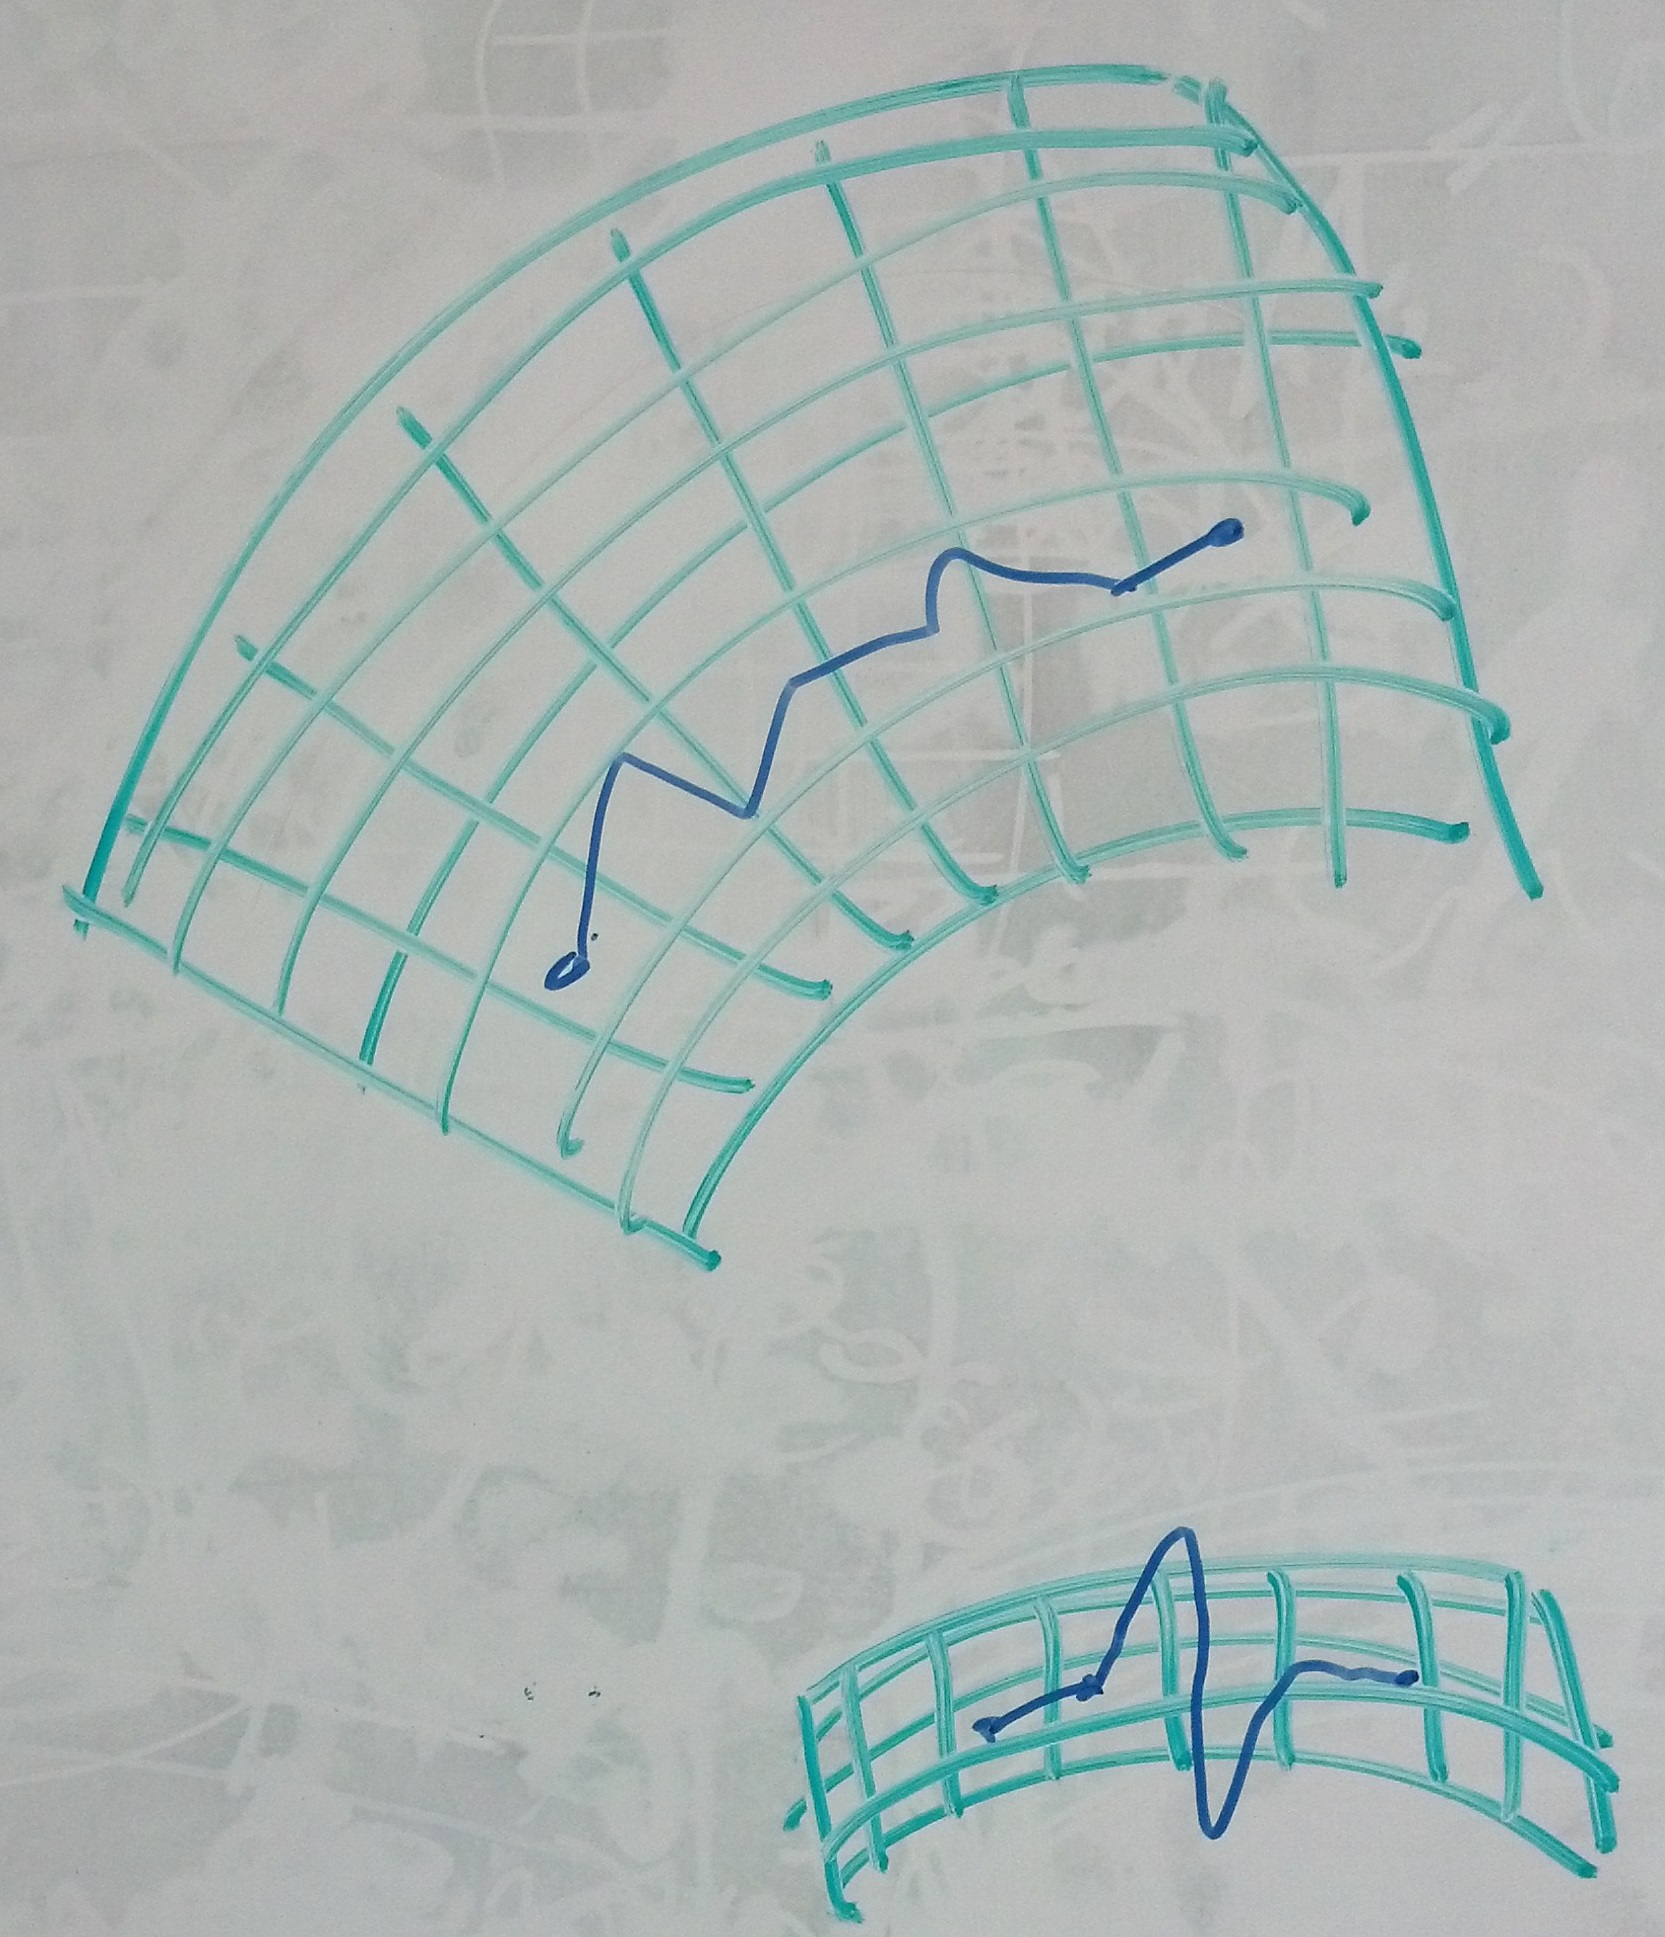
\includegraphics[width=\columnwidth]{pathaboveandbelow.jpg}
\caption{Path above and below surface}
\label{pathsAboveAndBelow}
\end{figure}

Our path is defined as a starting point $p$ and a set of $n$ segments $s_0,...,s_{n-1}$ where each segment is a vector with direction and magnitude. The starting point of $s_0$ is $p_0$ and for all $i>0$ the starting point of $s_i$ is the ending point of $s_{i-1}$. The mesh is a triangular manifold mesh **MAKE SURE THIS IS PREVIOUSLY ESTABLISHED**. \\
\\
After finding how the first segment follows the mesh, we will have a new start point on the mesh as well as $n-1$ segments that need to be projected onto the mesh. We can thus have an algorithm that finds a projection for a single vector and starting point and then recursively computes the rest of the path, below:.\\
\\
Project( $p$, $\{s_0,s_1,...,s_{n-1}\}$,$M$ ):\\
-Project $s_0$ onto $M$\\
-Get new start point $p'$\\
-Project( $p'$, $\{s_1,...,s_{n-1}\}$,$M$)\\ 
\\
When we project the first segment, we want it to follow the geodesic path along the mesh. **JUSTIFY THIS**. We will therefore flatten the mesh around the local area that the segment traverses. We will denote $T$ as the triangle where the starting point lies. We will develop a secondary mesh $M_0$ that consists of $T$ and its neighbors. The triangles in $M_0$ will be rotated so that they lie on the same plane as $T$. \\
\\
We will let $v$ be the vector for our input segment, $N$ be the normal of $T$, and $E$ be the resultant vector that is both on the plane formed by $N$ and $v$ and has an acute angle with $v$. As can be observed in figure \ref{vectordiagram}, the following equation will then hold
\[
E + proj_N(v) = v
\]

\begin{figure}[ht]
\centering
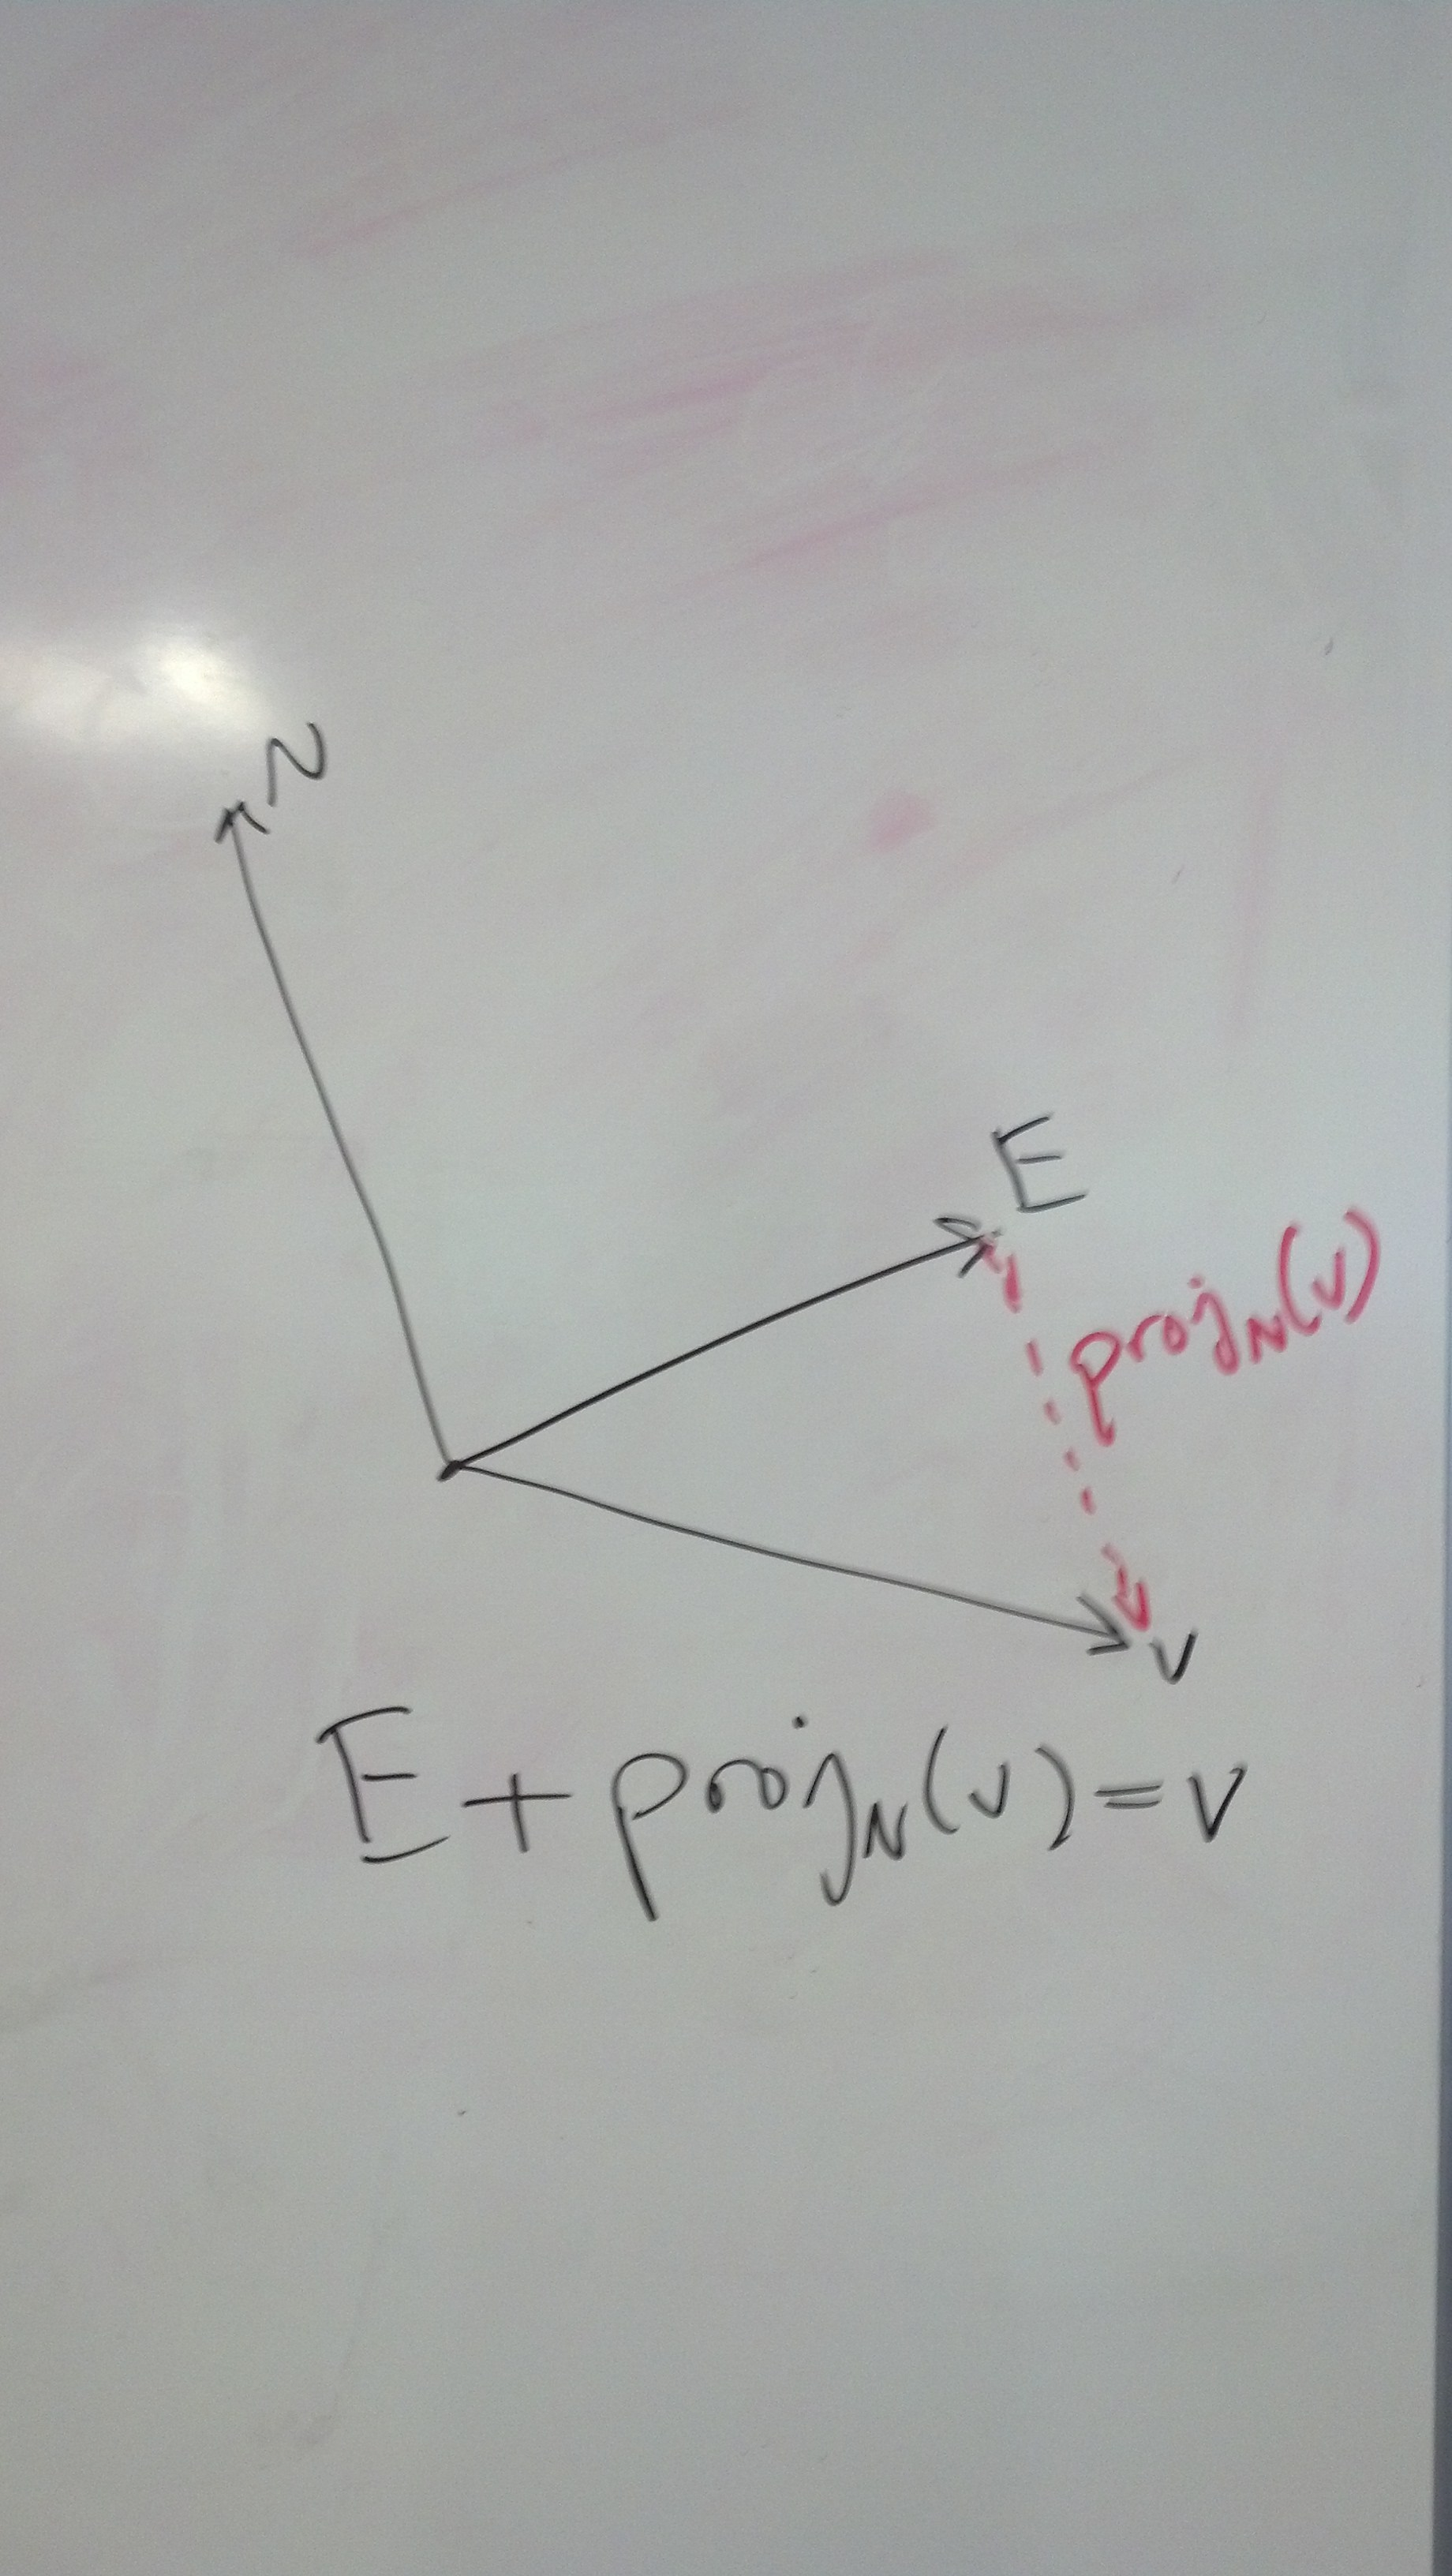
\includegraphics[width=\columnwidth]{vectordiagram.jpg}
\caption{The segment vector, normal, and projected vector}
\label{vectordiagram}
\end{figure}

Thus, the following equation will get us $E$
\[
E = v - proj_N(v)
\]
This can be further simplified to say
\[
E = v - N(v.N)
\]
We will draw $E$ on the mesh $M_0$. If the segment lies entirely inside $M_0$ as in Figure \ref{flatteningDiagram_oneTriangle}, then we are done. Otherwise, we will add triangles to $M_0$, rotate them to be on the same plane as $T$, and extend $E$ onto them, as in Figure \ref{flatteningDiagram_neighborhood}.By the manifold property, the flattening will always exists **JUSTIFY THIS** and this path will thus be a geodesic path **JUSTIFY THIS**. This will leave us with a series of connected points either on the interior or edges of each of the triangles. These points are computed in each triangle's coordinate system, so that the coordinates of these points in $M$ are easily computed and those coordinates are used to get the path that follows the mesh.\\
In the total, the algorithm takes in a starting point on the mesh $p$, a sequence of segments that starts from that point, and a triangular manifold mesh $M$. It outputs a sequence of points $\{ p_0, p_1, ... , p_m\}$ that lie on the mesh. The pseudo-code is in algorithm \ref{pseudocode}.\\
\\
\begin{algorithm}[t]
Input: Starting point $p_0$, Segments $s_0,...,s_m$, Mesh $M$\;
Set $p \leftarrow p_0$ \;
Initialize list $P$ of points and add $p_0$ to it \;
Set $T$ to be the triangle of $p_0$ \;
\For{each segment $s_i$ in order}{
	Set $N$ to be normal for $T$\;
	Clear $M_0$ and add $T$ to it \;
	Set $v$ to be the vector for $s_i$ \;
	Set $E \leftarrow v - N(v.N)$ \;
	Add Triangles to $M_0$ until $p+E$ is in $M_0$ \;
	Add points computed to $P$ \;
	Set $p$ $\leftarrow$ $p+E$ \;
}
\While{{\bf true}}{
		\While{top element of $E_M$ is positive}{
			Pop top element and move the data unit to its destination \;
			Update $E_M$ and $E_C$ \;
		}
		\eIf{there is more space for redundancy}{
		Pop top element and copy the data unit to its destination \;
		Update $E_M$ and $E_C$ \;
		}{{\bf break}}
}
\caption{Pseudo-code for our algorithm}
\label{pseudocode}
\end{algorithm}

\begin{figure}[ht]
\centering
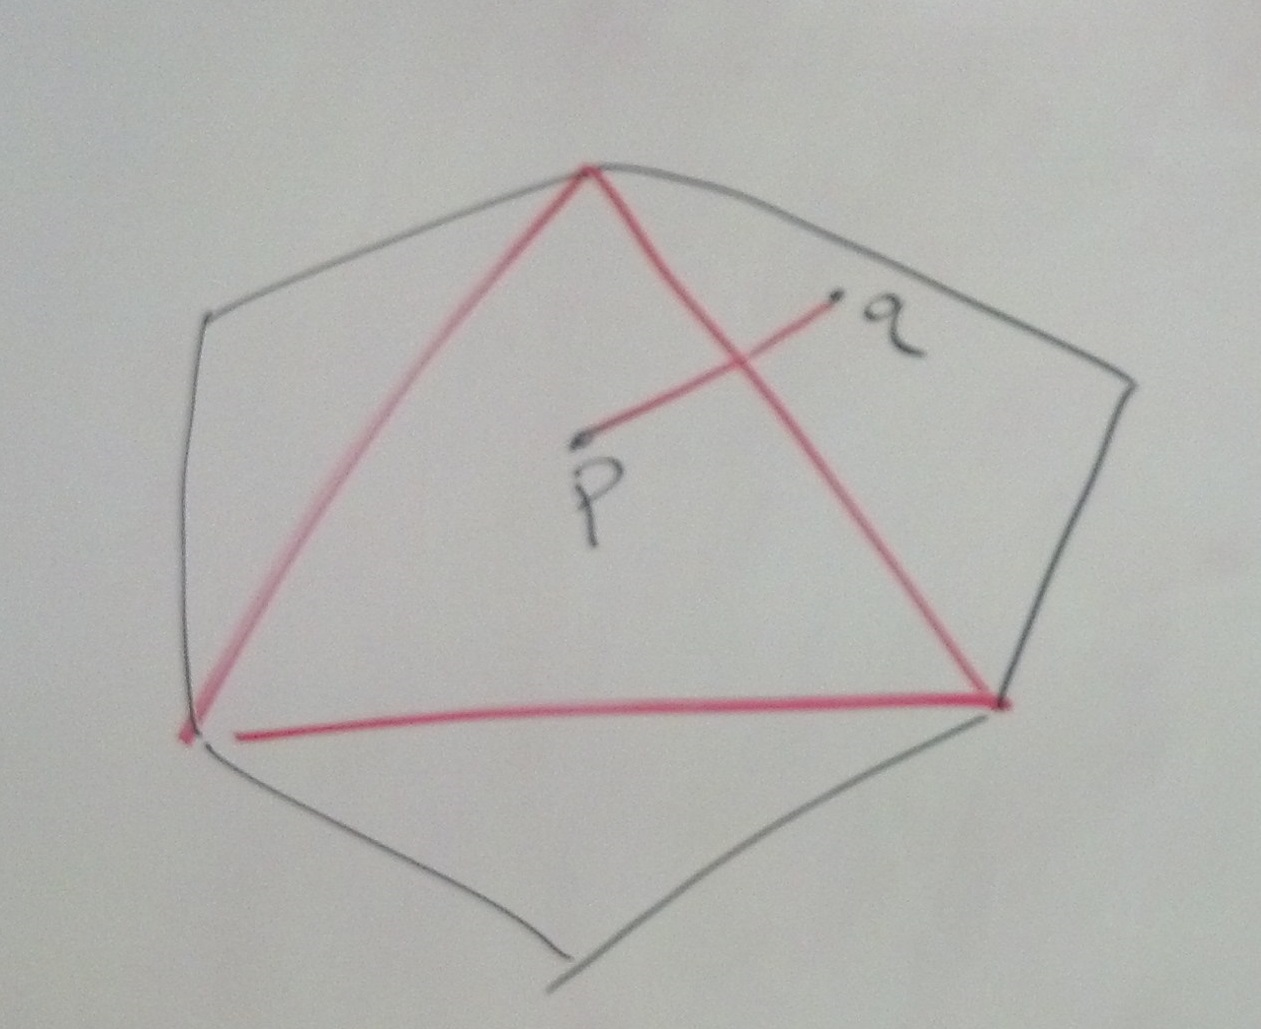
\includegraphics[width=\columnwidth]{flatteningdiagram_oneTriangleAndNeighbors.jpg}
\caption{The triangle at $p$ and its neighbors}
\label{flatteningDiagram_oneTriangle}
\end{figure}
\begin{figure}[ht]
\centering
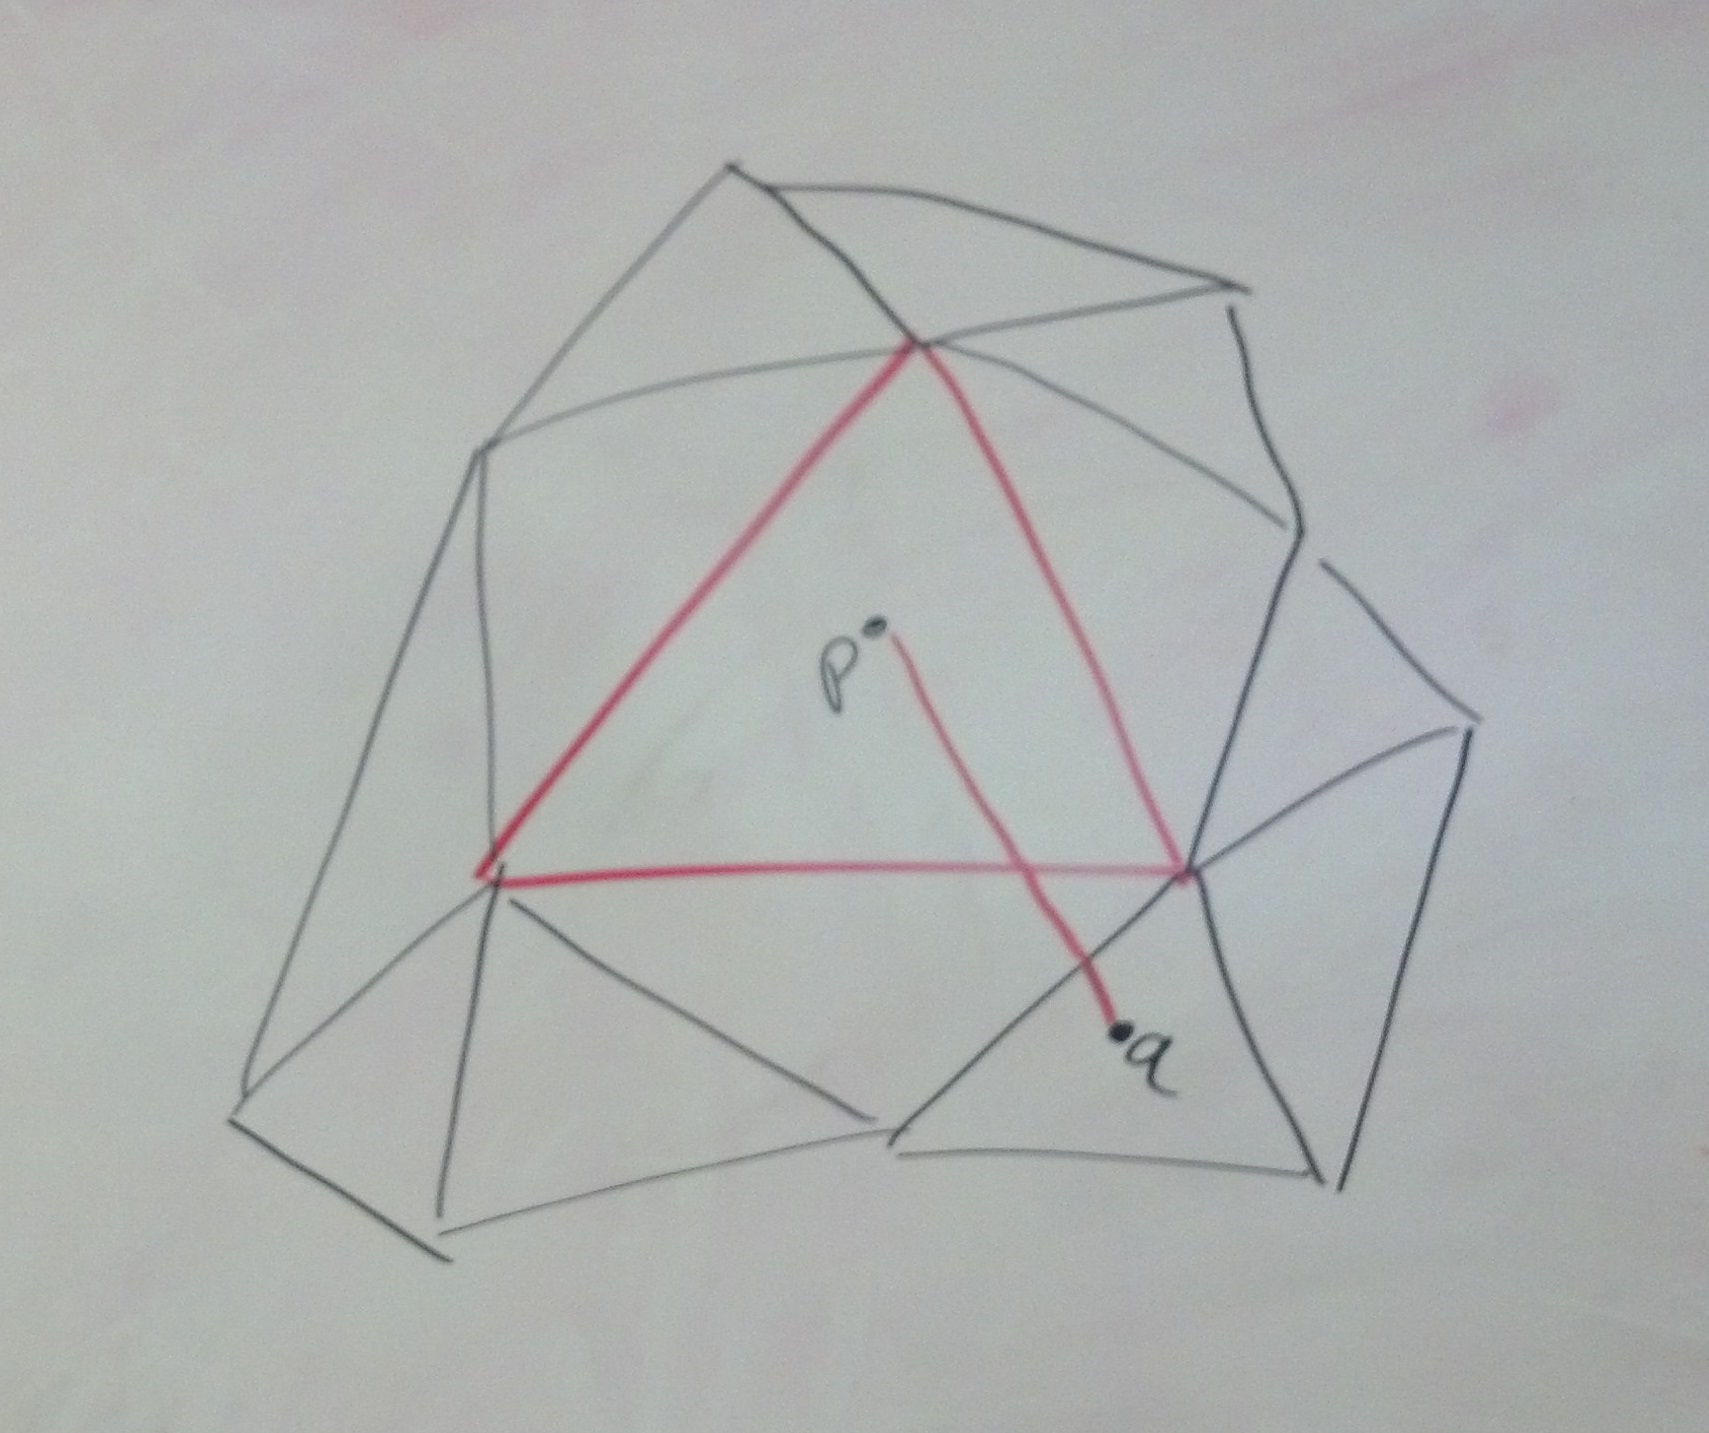
\includegraphics[width=\columnwidth]{flatteningdiagram_neighborhood.jpg}
\caption{The triangles in the neighborhood around $p$}
\label{flatteningDiagram_neighborhood}
\end{figure}

\subsection{Justification}

%In Theorem 9.10.11 of \ref{mathText}, the geodesic is defined to be the curve of shortest %length between two points on the surface. 
We have a recorded path and an algorithm to transform that to the surface. Because a path is a series of short segments, we just need to justify that algorithm for a single segment. Each segment of our path represents the distance and direction traveled in a very small amount of time. We are given a start point on the surface and vector and need to calculate the path on the surface. \\
\\
This tracking system is meant to be used with a system that rapidly samples the location of a probe. This means that an individual segment is thus quite short. Additionally, the surface is generally assumed to a low curvature. The surface we are tracking over must be a manifold. The combination of short segments and low curvature leads to the following assertion that will be used in my justification: {\it If $\epsilon$ is the length of the segment, then the $\epsilon$-neighborhood around the start point of the segment is homeomorphic to $R^2$}. This is illustrated in figure \ref{manifolddiagram}.\\
\\
\begin{figure}[ht]
\centering
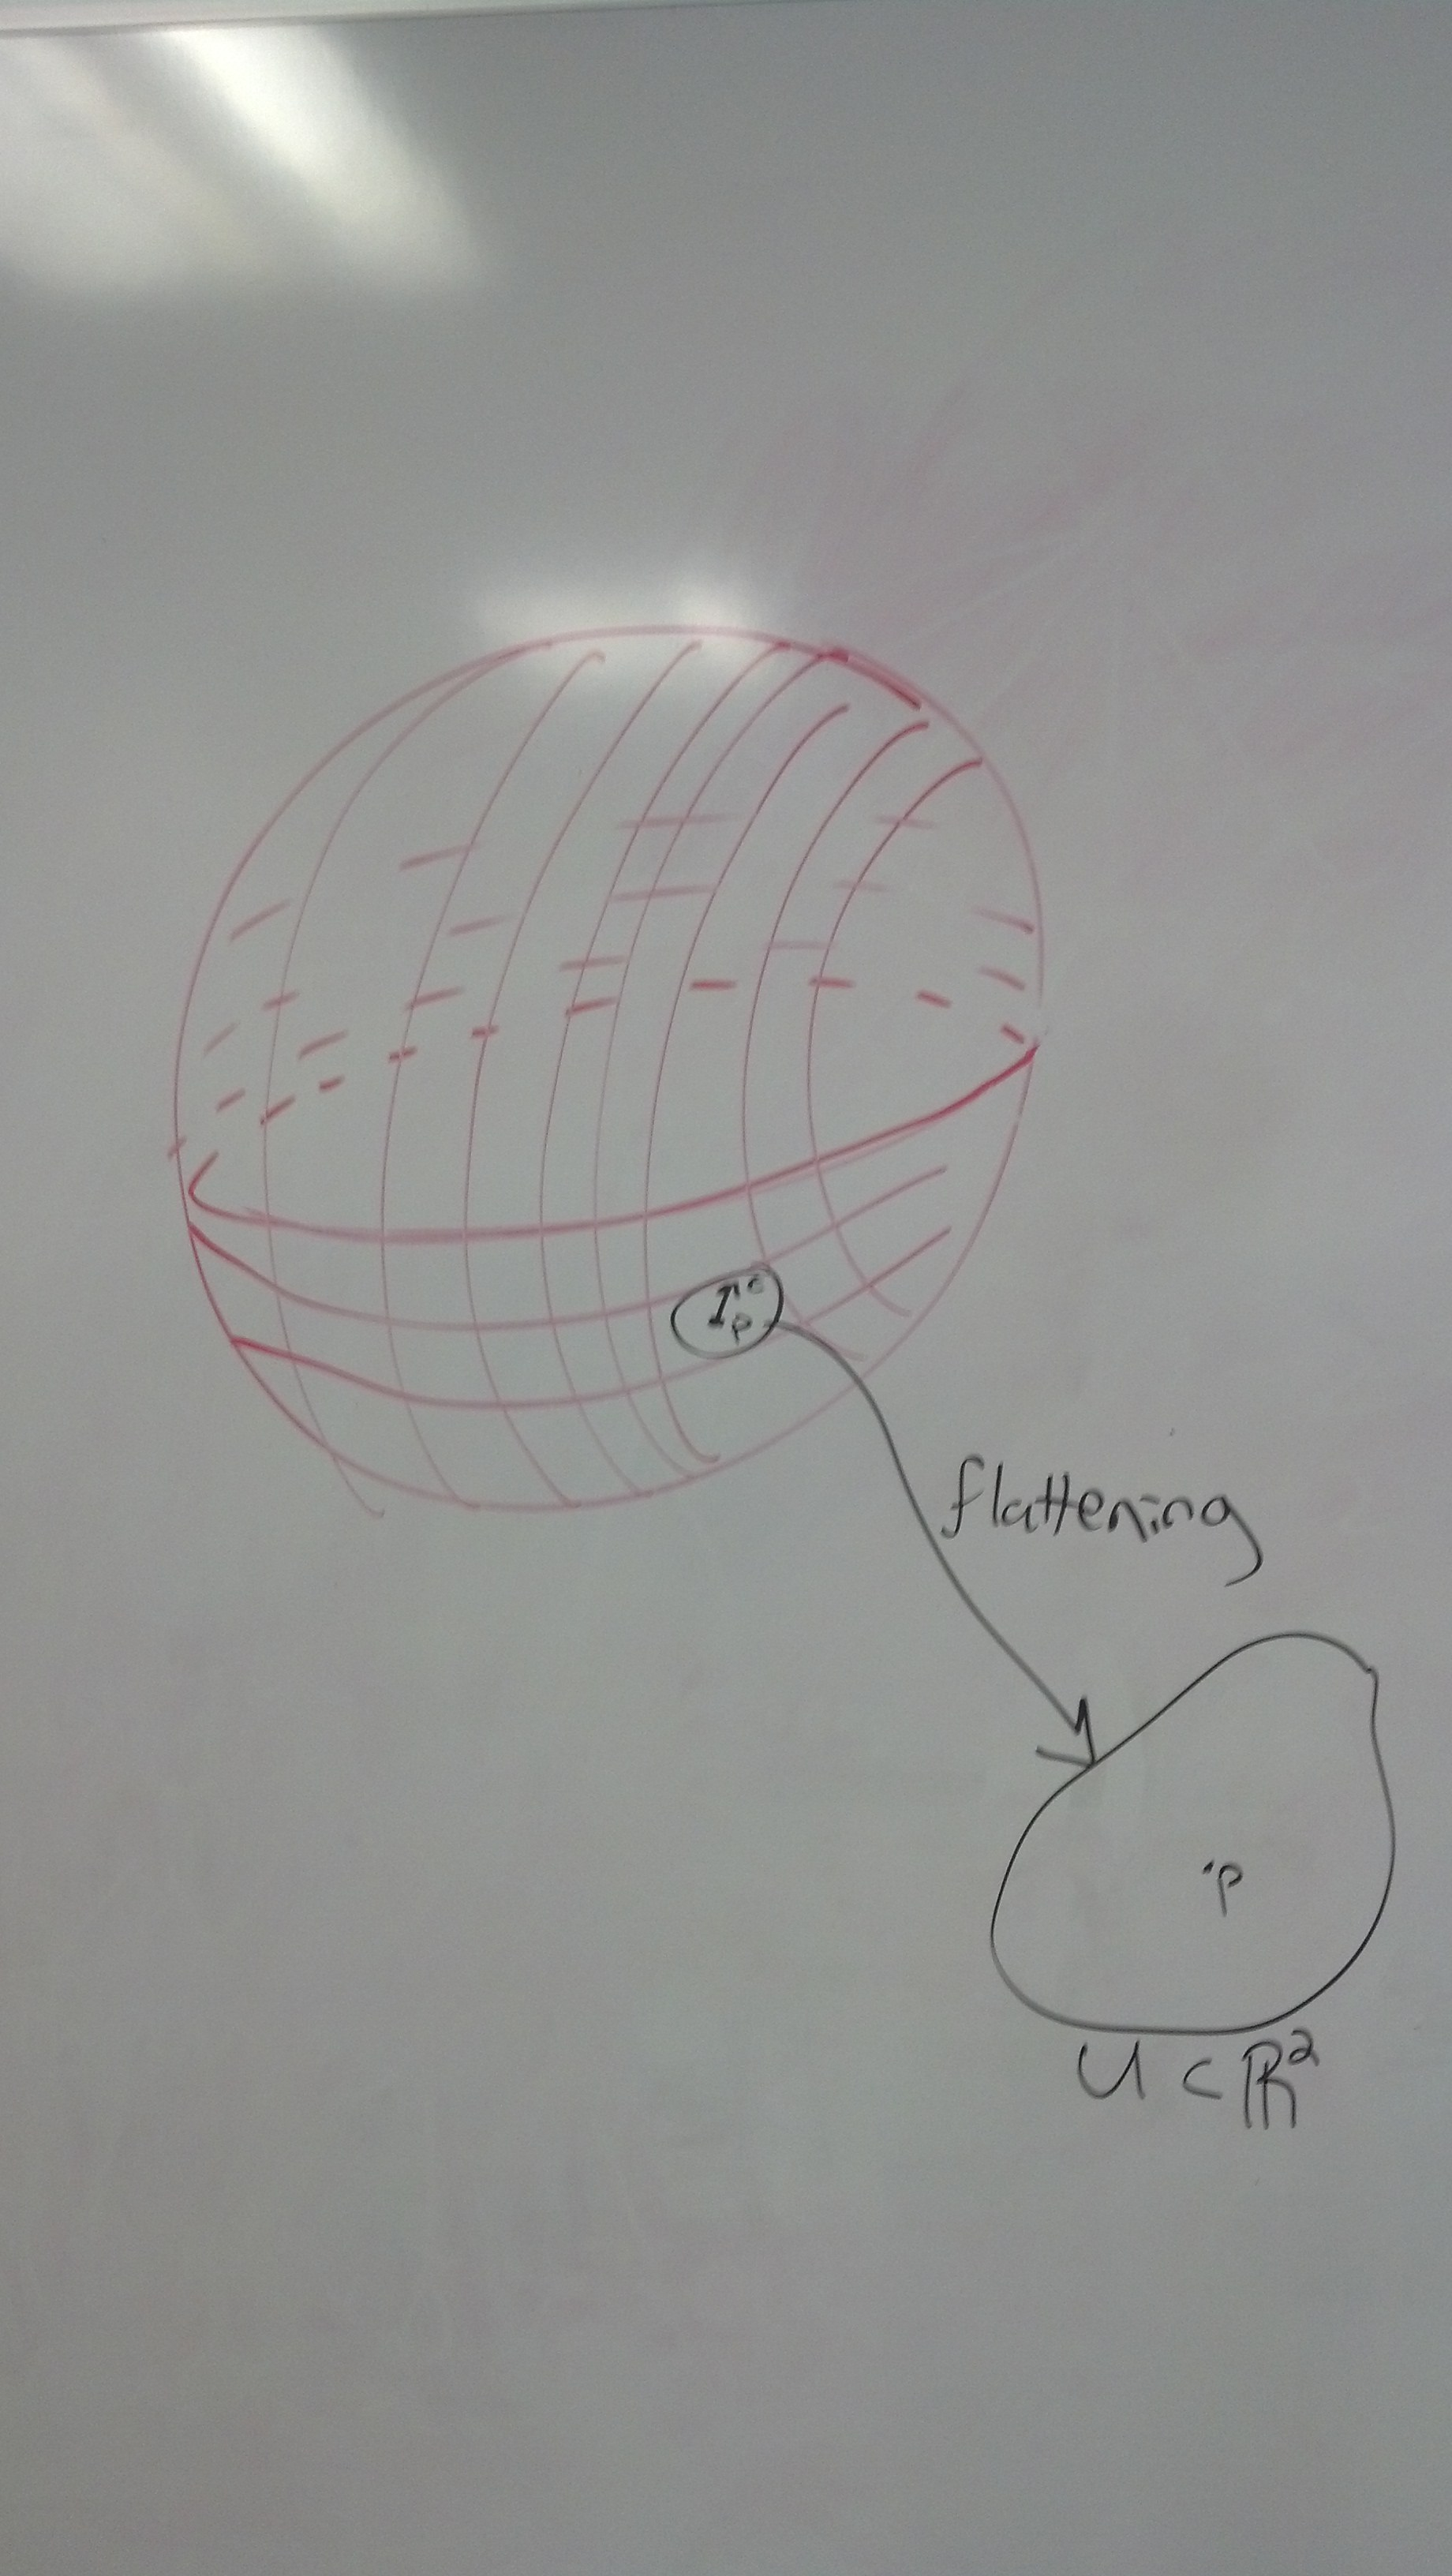
\includegraphics[width=\columnwidth]{manifolddiagram.jpg}
\caption{The manifold with its $\epsilon$ neighborhood at a point $p$}
\label{manifolddiagram}
\end{figure}
Because the sampling rate was so rapid, we can assert that between samples, a straight line on the surface was followed. We can thus assert the following: {\it The segment follows the geodesic path from start to end point along the surface}. We do not have the end point on the surface but when we assert an end point later, the path that was calculated will be the geodesic path from start to end point along the surface. \\
\\
**IMPROVE THIS** Because the output of our algorithm is the path along the surface, we must make sure the orientation of the probe along the surface is improved. We thus assert that we can only rotate the vector in the plane formed by the segment vector and the normal. Rotating it in any other plane would change the orientation along the surface. The transformed vector still needs to be perpendicular to the normal, thus we will have two options for it. We must pick the option that leaves us with an acute angle between the transformed vector and original vector as picking the other one would also change the orientation. We have now justified the following facts that were used to make the formula for the transformed segment vector: \\
{\it The transformed vector must be rotated along the same plane as the normal and the original vector}\\
{\it The transformed vector and original vector must form an acute angle}
\\
\\
We have now justified the direction of our transformed vector. We need to preserve arc-length of the path hence the length of our transformed vector will be the same as the length of the segment vector. This could have the implication that the transformed vector goes past the triangle it is located on. If that is the case, then we cut off the segment at the edge and transform the remaining vector. We repeat this procedure until a segment lies entirely in a triangle. \\
\\
We finally need to justify that this produces the geodesic in our desired direction on the surface. In the case where the entire segment can be put into its current triangle, this is trivial as we are following the straight line along that part of the surface. We thus need to justify the case where we traverse multiple triangles. Due to the homeomorphism mentioned above, we can locally flatten the triangles and avoid the gaps and overlaps that sometimes happen when there is mesh flattening. At each point in the algorithm, we are putting the path on the plane in the direction of the segment. Thus it is in the straight line direction. This means that when you flatten the triangles, the path will be a straight line in the direction we wanted. It will thus be the shortest path between the start and end points. This is illustrated in figure \ref{flatteningDiagram_oneTriangle} and figure \ref{flatteningDiagram_neighborhood}. 





\bibliographystyle{acmsiggraph}
\bibliography{trackingRefs}

\end{document}
